\newpage
\section{HM.TimerBasedScheduler}
Die benötigten Funktionen und Klassen, zur Realisierung des in Abschnitt \ref{sec:Gesamtkonzept} beschriebenen Konzepts zur Verwaltung aller wiederkehrenden Aufgaben, werden im Verzeichnis \textit{HM.TimerBasedScheduler} organisiert. Hierbei steht im Mittelpunkt die Verwendung der \textit{Timer}-Klasse. Diese wird vom .Net Framework bereitgestellt, und ermöglicht die Erzeugung von Ereignissen, nach Ablaufen einer vordefinierten Zeit. Auch das Erzeugen wiederkehrender Ereignisse ist mittels dieser Klasse möglich. \cite{SystemTimers}\\
Das \textit{IJob}-Interface definiert hierbei zunächst die Schnittstelle eines Jobs. Abgeleitet von diesem Interface, implementiert die abstrakte \textit{JobBase}, die Basis eines Jobs. Diese kann nicht direkt instanziiert werde und definiert lediglich die gemeinsamen Eigenschaften der \textit{Job}-Klassen.\\ 
Die \textit{JobBase} enthält einen \textit{Timer}, so wie eine \textit{Configuration} Objekt. Diese werden im Konstruktor der Klasse instanziiert und eingestellt. Das \textit{Configuration} Objekt wird hierbei über die \textit{ConfigurationReader}-Klasse erzeugt und mit den in der Konfigurationsdatei hinterlegten Einstellungen beschrieben. Dem \textit{Timer}-Objekt wird zunächst das \textit{Exceute} der \textit{JobBase} Klasse zugewiesen. Dieses wird aufgerufen, sobald der Timer abgelaufen ist. Zudem wird die \textit{AutoReset}-Property des Objekts aktiviert. Sie bewirkt einen automatischen Neustart des Timers, sobald dieser abgelaufen ist.\\
Im Anschluss werden die \textit{ReadingJob}-, \textit{CurrentSystemStatusJob}- und \textit{SystemStatusHistoryJob}-Klassen von der \textit{JobBase}-Klasse abgeleitet. In diesen werden die Spezifischen Aufgaben jedes Jobs implementiert. Die auszuführende Aufgabe wird in den jeweiligen \textit{Esecute}-Events der Klassen implementiert.\\

\subsection{ReadingJob}
\begin{wrapfigure}{r}{0.4\textwidth}
    \vspace{-2cm}
    \begin{center}
      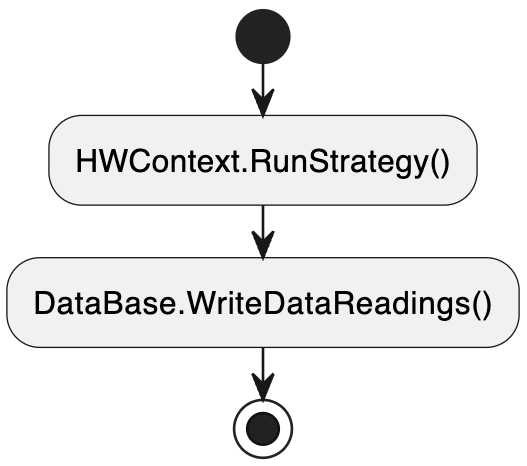
\includegraphics[width=0.35\textwidth]{ReadingJobExecute.png}
    \end{center}
    \vspace{-0.5cm}
    \caption{Ablaufdiagram des Execute Events der \textit{ReadingJob}-Klasse}
    \label{fig:ReadingJobExecute}
    \vspace{-1cm}
  \end{wrapfigure}
Die \textit{ReadingJob}-Klasse referenziert die Verzeichnisse \textit{HM.HWServices} und \textit{HM.DBServices}. Hierbei werden im Konstruktor der Klasse Datenbank so wie Auswertestrategie (Siehe \ref{sec:AuslesenHardware}) instanziiert. Das \textit{Configuration}-Objekt enthält die hierzu notwendigen Informationen, wie zum Beispiel Name der Datenbank, Hardwarekonfiguration oder Zeitintervall des entsprechenden Jobs.\\
Über den die \textit{Context}-Klasse des \textit{HM.HWServices} Verzeichnisses wird zunächst, abhängig von angegebener Zielplattform, die passende Strategieklasse geladen. Hierzu wird die \textit{SetStrategy()} Funktion der \textit{Context}-Klasse aufgerufen. Anschließend wird über die Instantiierung der \textit{SQLiteWrapper}-Klasse eine Verbindung zur Datenbank aufgebaut. Das in der Konfigurationsdatei hinterlegte Zeitintervall des \textit{ReadingJob} wird in millisekunden umgewandelt und anschließend der \textit{Interval}-Property des Timers übergeben.\\
Die Logik zur Datenerfassung wird im \textit{Execute}-Event der Klasse implementiert. Hierzu wird zunächst die \textit{RunStrategy()}-Funktion des \textit{Context} aufgerufen. Anschließend werden die Sensorwerte über die \textit{WriteDataReadings()}-Funktion des \textit{SQLiteWrapper} in die Datenbank geschrieben. (Siehe Abbildung \ref{fig:ReadingJobExecute})

\subsection{CurrentSystemStatusJob}
\begin{wrapfigure}{r}{0.3\textwidth}
    \vspace{-1.2cm}
    \begin{center}
      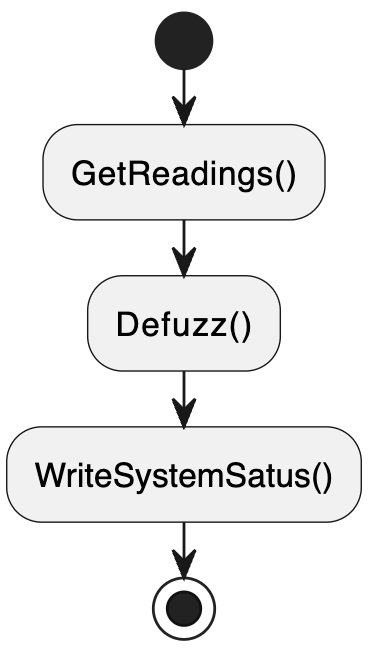
\includegraphics[width=0.3\textwidth]{CurrentSystemStatusExecute.png}
    \end{center}
    \vspace{-0.5cm}
    \caption{Ablaufdiagram des Execute Events der \textit{CurrentSystemStatusJob}-Klasse}
    \label{fig:CurrentSystemStatusJob}
  \end{wrapfigure}
Die \textit{CurrentSystemStatusJob}-Klasse referenziert die Verzeichnisse \textit{HM.ScoringModel} und \textit{HM.DBServices}. Im Konstruktor werden zunächst die Datenbank und Timer der Klasse instanziiert. Anschließend wird abhängig von der in der Konfigurationsdatei hinterlegten Hardwarekonfiguration die passende \textit{FuzzyLogic}-Klasse geladen (Siehe \ref{fig:ScoringModel}). Hierbei wird zudem auch die passende \textit{FuzzyLogicMTBF}-Klasse, zur Ermittlung des Temperaturabhängigen \ac{mtbf} des Systems, geladen.\\
Die Logik der Systemauswertung wird anschließend, im \textit{Execute}-Event der Klasse zusammengeführt. Die \textit{GetReadings()} Funktion liest zunächst die benötigten Datensätze aus der Datenbank. Anschließend werden diese über die \textit{Defuzz()} Funktion durch die zuvor konfigurierte Fuzzylogic verarbeitet. Das Ergebnis der Systembewertung wird im Anschluss über die \textit{WriteSystemStatus()} Funktion in der Datenbank gespeichert.\\
Die \textit{CurrentSystemStatusJob}-Klasse ermittelt auf diesem Weg zum einen den aktuellen Systemstatus der Plattform. Zusätzlich speichert sie die temperaturabhängige \ac{mtbf} Bewertung des Systems zur Ermittelung der Systemzuverlässigkeit. (Siehe Abbildung \ref{fig:CurrentSystemStatusJob})   

\subsection{SystemStatusHistoryJob}
\begin{wrapfigure}{r}{0.3\textwidth}
    \vspace{-1.2cm}
    \begin{center}
      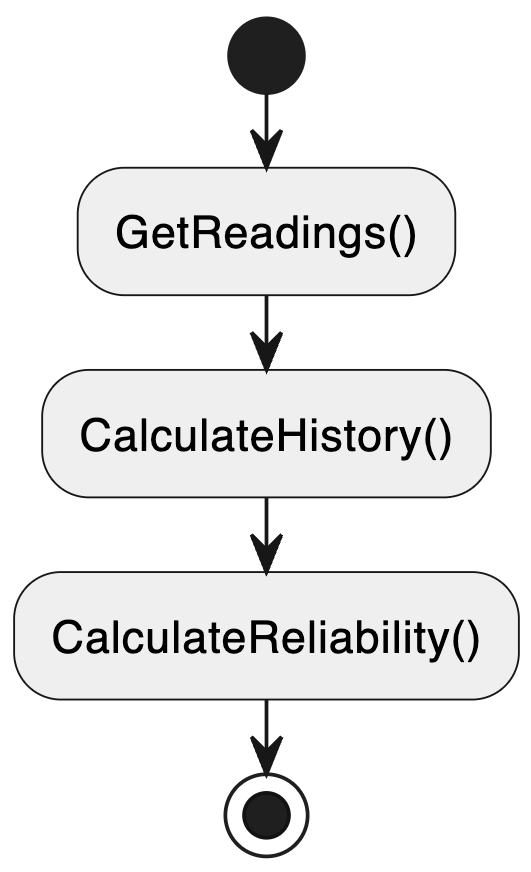
\includegraphics[width=0.2\textwidth]{SystemStatusHistoryJobAblauf.png}
    \end{center}
    \vspace{-0.5cm}
    \caption{Ablaufdiagram des Execute Events der \textit{SystemStatusHistoryJob}-Klasse}
    \label{fig:SystemStatusHistoryJob}
  \end{wrapfigure}
Wie auch die \textit{CurrentSystemStatusJob}-Klasse referenziert die \textit{SystemStatusHistoryJob}-Klasse die Verzeichnisse \textit{HM.ScoringModel} und \textit{HM.DBServices}. Hierbei werden die \textit{SQLiteWrapper}-, \textit{Timer}- und \textit{StatusHistory}-Klassen im Konstruktor der Klasse Instanziiert. Da die Plattformabhängigen Berechnungen der benötigten Werte bereits in den Klassen zuvor durchgeführt werden, wird im Konstruktor dieser klasse lediglich Datenbankname und Zeitintervall aus der Konfigurationsdatei geladen.\\
Im \textit{Execute}-Event der Klasse werden zunächst alle benötigten Werte zur Berechnung von Systemstatus Historie und Zuverlässigkeit aus der Datenbank entnommen. Anschließend wird über die \textit{CalculateHistory()} Funktion er \textit{StatusHistory}-Klasse die Systemstatus Historie berechnet. Diese wird in der \textit{HistorySystemStatus} Tabelle der Datenbank abgelegt. Des Weiteren wird über die \textit{CalculateReliabilty()} Funktion der Klasse die Systemzuverlässigkeit berechnet, welche in der \textit{SystemReliabilty} Tabelle der Datenbank abgespeichert wird. (Siehe Abbildung \ref{fig:SystemStatusHistoryJob})
  